\documentclass[a3paper, landscape, border=1cm]{standalone}

\usepackage{tikz}
%\usetikzlibrary{arrows.meta, shapes.geometric, decorations.pathreplacing}  % Load libraries for arrows, shapes, and decorations

\begin{document}

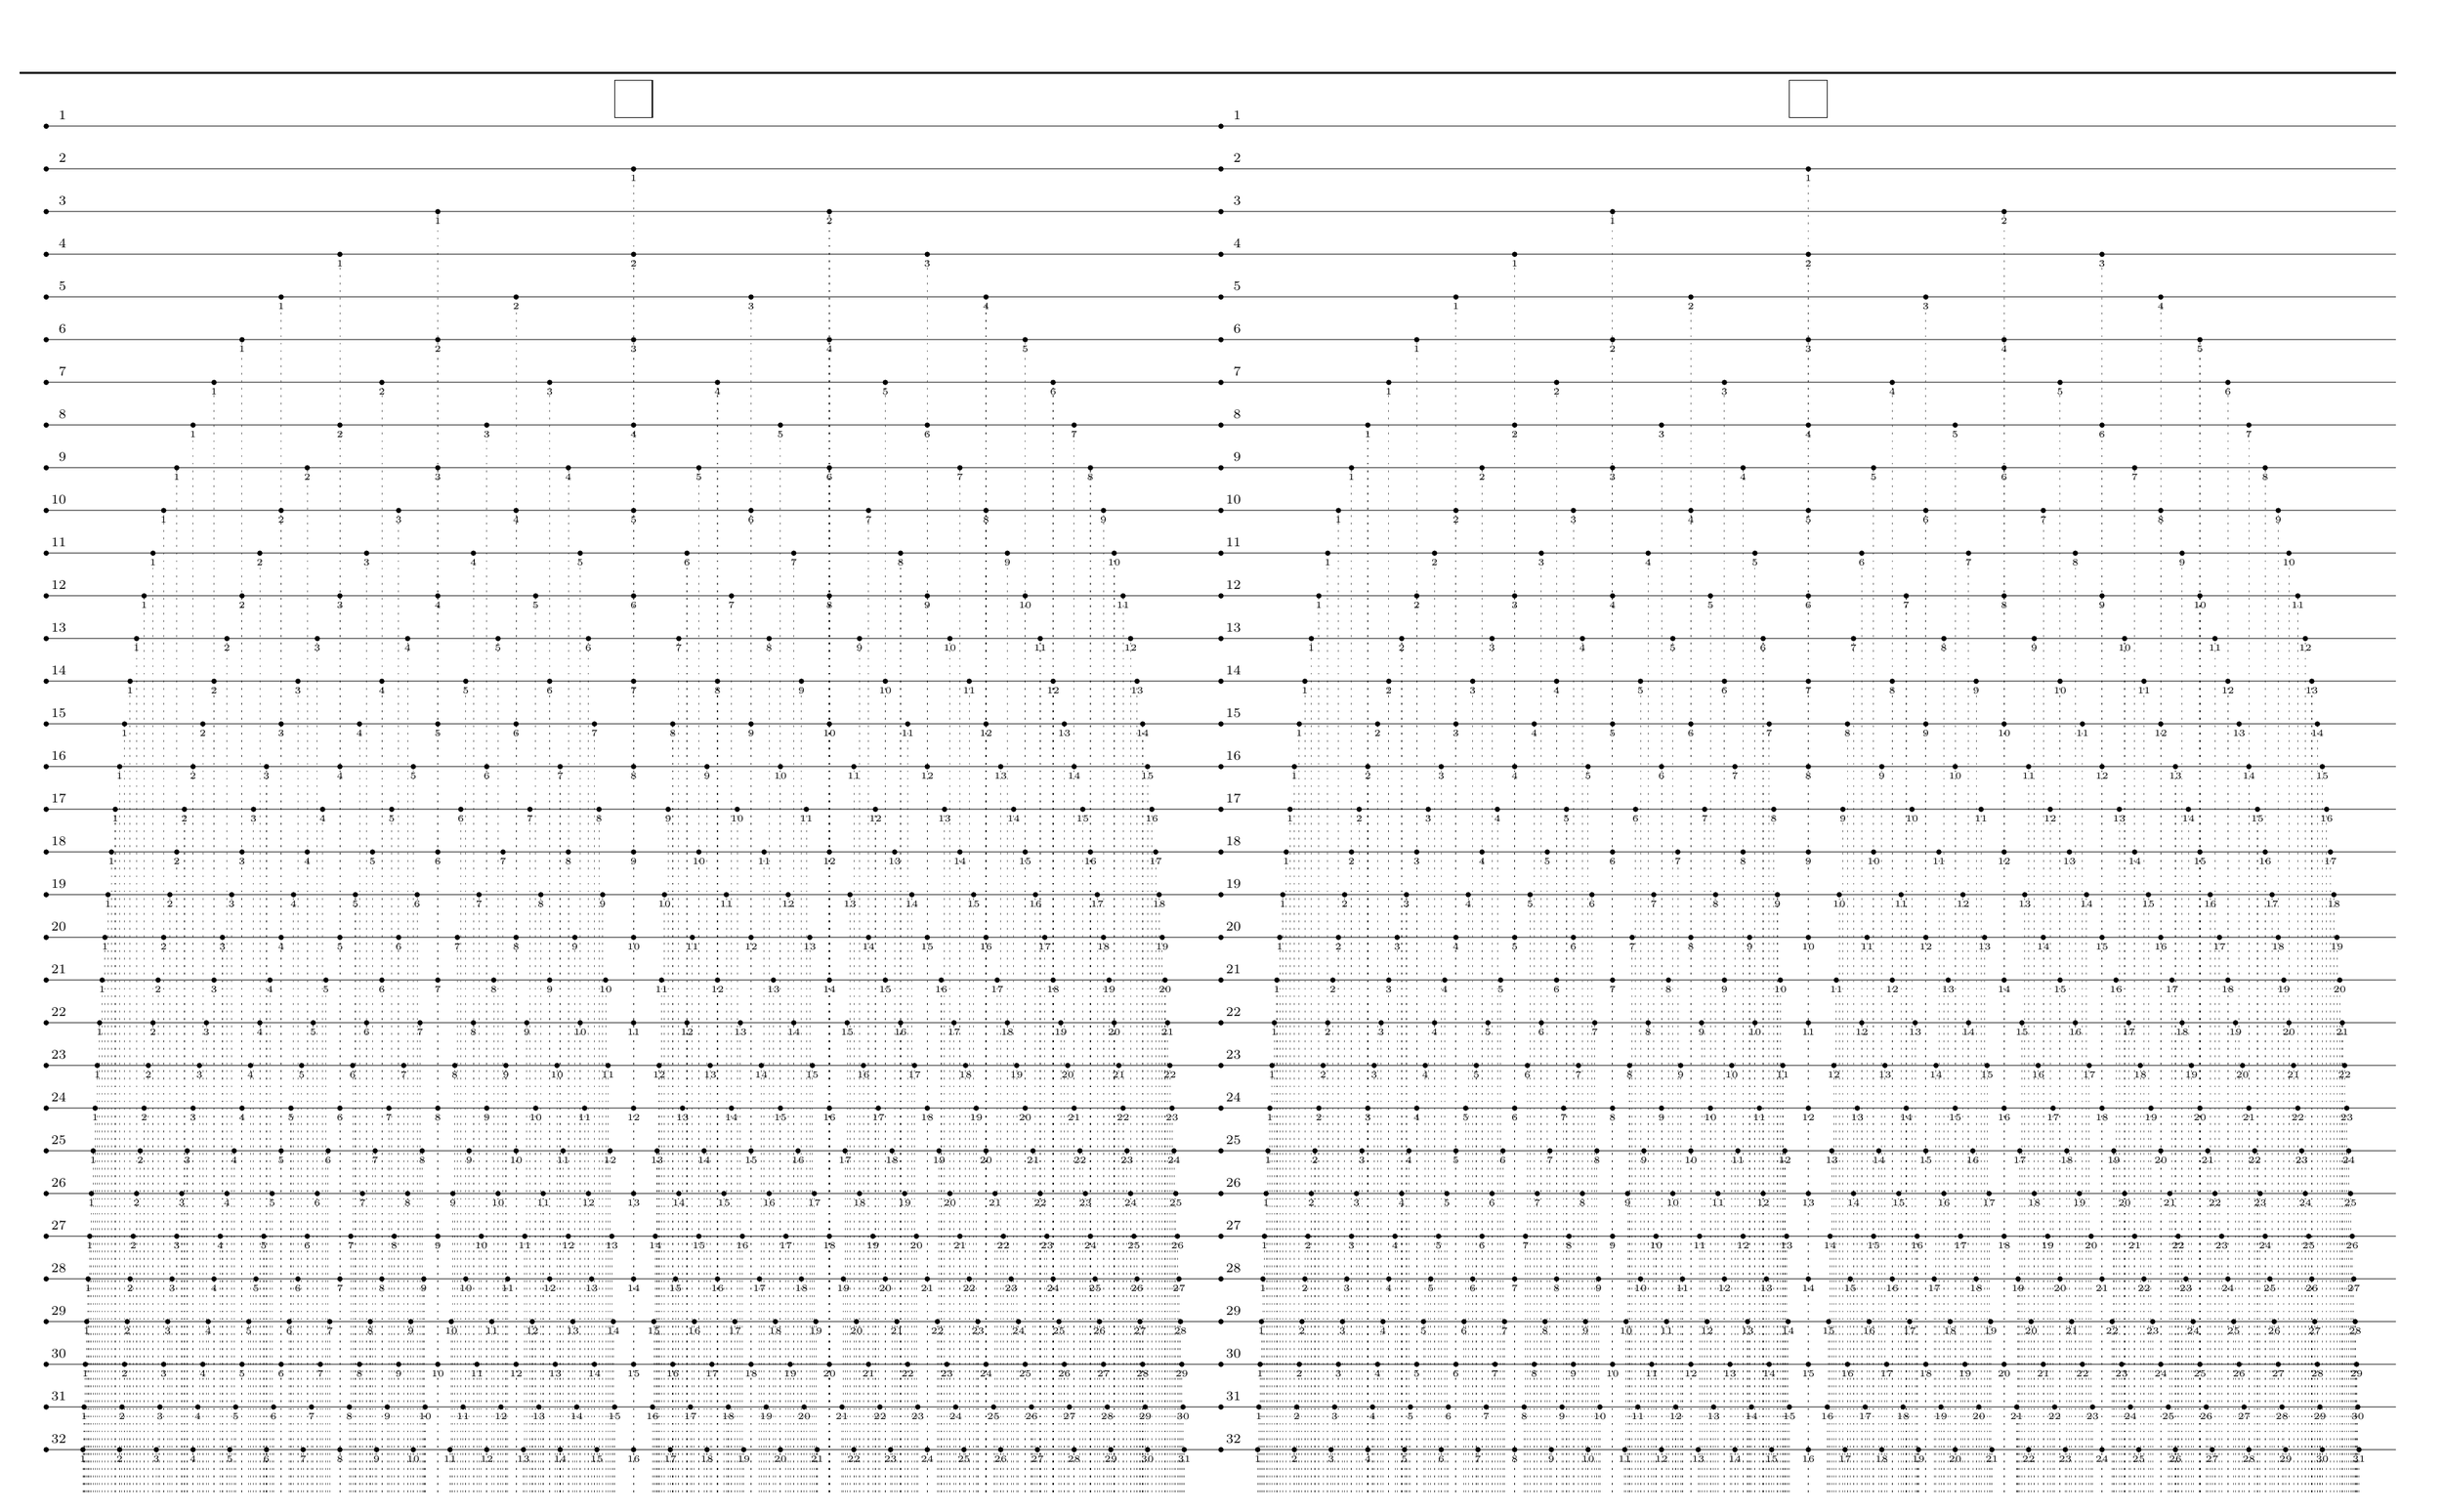
\begin{tikzpicture}

% General parameters
\def\length{22}           % Length of the line
\def\spacing{0.8}         % Distance between lines
\def\numLines{32}         % Number of lines
\def\numUnits{2}          % Number of units (number of grids)
\def\frameMargin{0.5}     % Margin for the frame
\def\topSpace{1}          % Extra space above the top frame
\def\timeLineSpace{.2}    % Space between the frame and the lines
\def\gridWidth{\length + 2*\frameMargin}  % Total width of the grid (including margins)
\def\pointRadius{1.4pt}

% Loop to repeat the drawing across the x-axis
\foreach \k in {0,...,\numexpr\numUnits-1\relax} {    % Horizontal shift for each grid
    \begin{scope}[shift={(\k*\gridWidth,0)}]

    % Top frame
    \draw[thick] (-\frameMargin, -\topSpace) -- (\length, -\topSpace);
    \draw[thick, opacity=0] (-\frameMargin, 0) -- (\length, 0);

    % Loop to draw the lines
    \foreach \i in {1,...,\numLines} {
        % Coordinates of the line
        \def\y{-\i*\spacing-\topSpace-\timeLineSpace}  % The y-coordinate decreases each time, including extra space

        % Draw the normal line with opacity
        \draw[thick, color=black, opacity=.5] (0, \y) -- (\length, \y);

        % Calculate the divisions
        \ifnum\i>1
           \pgfmathsetmacro\division{\i-1}  % Number of divisions
            \foreach \j in {1,...,\division} {
                \pgfmathsetmacro\xPos{\j*\length/(\division+1)}  % Position of the point

                \node (point-\k-\i-\j) at (\xPos, \y) [circle, fill, inner sep = 1pt] {};  % Draw the point with varying color
                % Add label below the point
                \node[below, font=\tiny] at (\xPos, \y) {\j};

                % Draw the dashed vertical line passing through the point
                \draw[dashed, dash pattern=on 1pt off 3pt, opacity=.6] (\xPos, -\spacing*\numLines-\spacing-\timeLineSpace-\topSpace) -- (\xPos, \y); 
                % Add label above the point (\k-1-1) only once per \k cycle
                \ifnum\i=2
                    \ifnum\j=1
                        \node[draw, rectangle, above, font=\large, inner sep=10pt, minimum width=1em, minimum height=1em] at (\xPos, \y + .95) {};%{$\k$};
                    \fi
                \fi

                }
        \fi
        % Draw the label on the left of each line
        \node[anchor=east,font=\scriptsize] at (+.5, \y+.2) {\i};
        % Draw a point at the beginning of each line
        \node (point-\k-\i-0) at (0, \y)  [circle, fill, inner sep = 1pt] {};


        }

    % Bottom frame (not visible for now, with opacity=0)
    \draw[thick, opacity=0] (-\frameMargin, -\spacing*\numLines-\spacing-\timeLineSpace-\topSpace) -- (\length+\frameMargin,  -\spacing*\numLines-\spacing-\timeLineSpace-\topSpace);
    \end{scope}
}

\end{tikzpicture}

\end{document}
